\documentclass{standalone}
\usepackage{tikz}
\usetikzlibrary{patterns, positioning}

\begin{document}
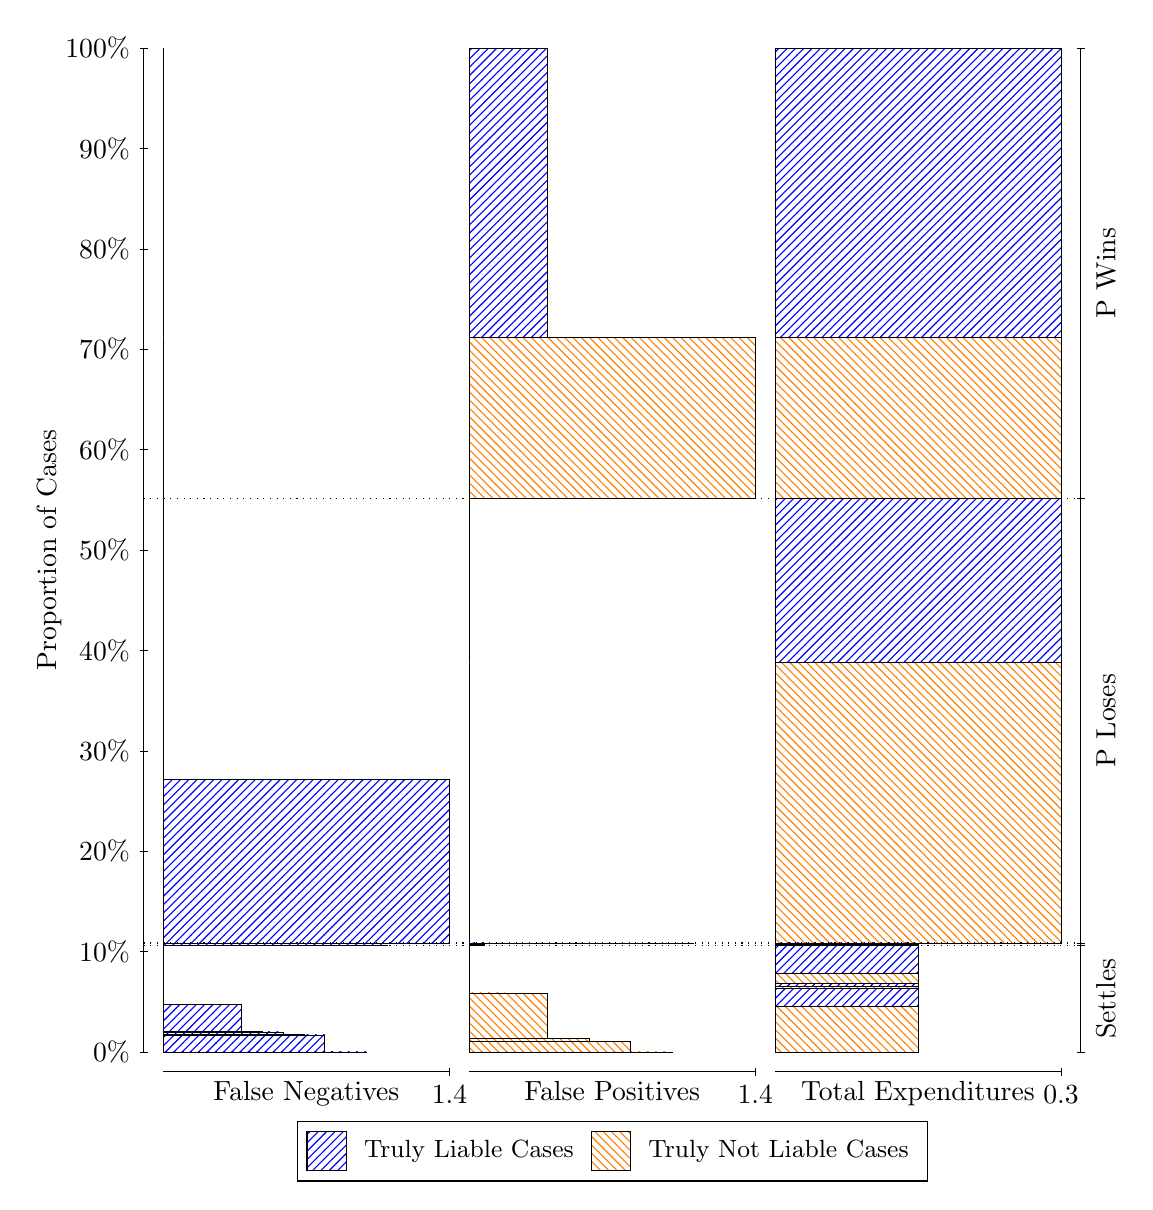
\begin{tikzpicture}
\draw[black, very thin] (1.5,1.75) -- (1.5,14.5);
\node[rotate=90, anchor=center] at (0.3, 8.125) {Proportion of Cases};
\draw[black, very thin] (1.45,1.75) -- (1.55,1.75);
\node[anchor=east] at (1.45, 1.75) {0\%};
\draw[black, very thin] (1.45,3.025) -- (1.55,3.025);
\node[anchor=east] at (1.45, 3.025) {10\%};
\draw[black, very thin] (1.45,4.3) -- (1.55,4.3);
\node[anchor=east] at (1.45, 4.3) {20\%};
\draw[black, very thin] (1.45,5.575) -- (1.55,5.575);
\node[anchor=east] at (1.45, 5.575) {30\%};
\draw[black, very thin] (1.45,6.85) -- (1.55,6.85);
\node[anchor=east] at (1.45, 6.85) {40\%};
\draw[black, very thin] (1.45,8.125) -- (1.55,8.125);
\node[anchor=east] at (1.45, 8.125) {50\%};
\draw[black, very thin] (1.45,9.4) -- (1.55,9.4);
\node[anchor=east] at (1.45, 9.4) {60\%};
\draw[black, very thin] (1.45,10.675) -- (1.55,10.675);
\node[anchor=east] at (1.45, 10.675) {70\%};
\draw[black, very thin] (1.45,11.95) -- (1.55,11.95);
\node[anchor=east] at (1.45, 11.95) {80\%};
\draw[black, very thin] (1.45,13.225) -- (1.55,13.225);
\node[anchor=east] at (1.45, 13.225) {90\%};
\draw[black, very thin] (1.45,14.5) -- (1.55,14.5);
\node[anchor=east] at (1.45, 14.5) {100\%};

\draw[black, very thin] (13.4,1.75) -- (13.4,14.5);
\draw[black, very thin] (13.35,1.75) -- (13.45,1.75);
\node[anchor=west] at (13.35, 1.75) {};
\draw[black, very thin] (13.35,3.105) -- (13.45,3.105);
\node[anchor=west] at (13.35, 3.105) {};
\draw[black, very thin] (13.35,3.1256) -- (13.45,3.1256);
\node[anchor=west] at (13.35, 3.1256) {};
\draw[black, very thin] (13.35,3.1363) -- (13.45,3.1363);
\node[anchor=west] at (13.35, 3.1363) {};
\draw[black, very thin] (13.35,8.7798) -- (13.45,8.7798);
\node[anchor=west] at (13.35, 8.7798) {};
\draw[black, very thin] (13.35,14.5) -- (13.45,14.5);
\node[anchor=west] at (13.35, 14.5) {};

\draw[black, very thin, pattern color=blue, pattern=north east lines] (1.75,1.75) rectangle (4.3264,1.7504);
\draw[black, very thin, pattern color=blue, pattern=north east lines] (1.75,1.7504) rectangle (4.0621,1.7512);
\draw[black, very thin, pattern color=blue, pattern=north east lines] (1.75,1.7512) rectangle (3.7979,1.9682);
\draw[black, very thin, pattern color=blue, pattern=north east lines] (1.75,1.9682) rectangle (3.5336,1.9727);
\draw[black, very thin, pattern color=blue, pattern=north east lines] (1.75,1.9727) rectangle (3.2694,2.0041);
\draw[black, very thin, pattern color=blue, pattern=north east lines] (1.75,2.0041) rectangle (3.0052,2.013);
\draw[black, very thin, pattern color=blue, pattern=north east lines] (1.75,2.013) rectangle (2.7409,2.3528);
\draw[black, very thin, pattern color=blue, pattern=north east lines] (1.75,2.3528) rectangle (2.4767,2.3539);
\draw[black, very thin, pattern color=blue, pattern=north east lines] (1.75,2.3539) rectangle (2.2124,2.3548);
\draw[black, very thin, pattern color=orange, pattern=north west lines] (1.75,2.3548) rectangle (1.75,3.105);
\draw[black, very thin, pattern color=blue, pattern=north east lines] (1.75,3.105) rectangle (4.5906,3.1103);
\draw[black, very thin, pattern color=orange, pattern=north west lines] (1.75,3.1103) rectangle (1.75,3.1256);
\draw[black, very thin, pattern color=blue, pattern=north east lines] (1.75,3.1256) rectangle (1.9482,3.1335);
\draw[black, very thin, pattern color=orange, pattern=north west lines] (1.75,3.1335) rectangle (1.75,3.1363);
\draw[black, very thin, pattern color=blue, pattern=north east lines] (1.75,3.1363) rectangle (5.3833,5.2167);
\draw[black, very thin, pattern color=orange, pattern=north west lines] (1.75,5.2167) rectangle (1.75,8.7798);
\draw[black, very thin, pattern color=orange, pattern=north west lines] (1.75,8.7798) rectangle (1.75,10.823);
\draw[black, very thin, pattern color=blue, pattern=north east lines] (1.75,10.823) rectangle (1.75,14.5);
\draw[black, very thin, pattern color=orange, pattern=north west lines] (5.6333,1.75) rectangle (8.2097,1.7503);
\draw[black, very thin, pattern color=orange, pattern=north west lines] (5.6333,1.7503) rectangle (7.9455,1.7507);
\draw[black, very thin, pattern color=orange, pattern=north west lines] (5.6333,1.7507) rectangle (7.6812,1.8816);
\draw[black, very thin, pattern color=orange, pattern=north west lines] (5.6333,1.8816) rectangle (7.417,1.8871);
\draw[black, very thin, pattern color=orange, pattern=north west lines] (5.6333,1.8871) rectangle (7.1527,1.9186);
\draw[black, very thin, pattern color=orange, pattern=north west lines] (5.6333,1.9186) rectangle (6.8885,1.9265);
\draw[black, very thin, pattern color=orange, pattern=north west lines] (5.6333,1.9265) rectangle (6.8885,1.9266);
\draw[black, very thin, pattern color=orange, pattern=north west lines] (5.6333,1.9266) rectangle (6.6242,2.4968);
\draw[black, very thin, pattern color=orange, pattern=north west lines] (5.6333,2.4968) rectangle (6.36,2.4989);
\draw[black, very thin, pattern color=orange, pattern=north west lines] (5.6333,2.4989) rectangle (6.0958,2.5002);
\draw[black, very thin, pattern color=blue, pattern=north east lines] (5.6333,2.5002) rectangle (5.6333,3.105);
\draw[black, very thin, pattern color=orange, pattern=north west lines] (5.6333,3.105) rectangle (5.8315,3.1203);
\draw[black, very thin, pattern color=blue, pattern=north east lines] (5.6333,3.1203) rectangle (5.6333,3.1256);
\draw[black, very thin, pattern color=orange, pattern=north west lines] (5.6333,3.1256) rectangle (8.4739,3.1283);
\draw[black, very thin, pattern color=blue, pattern=north east lines] (5.6333,3.1283) rectangle (5.8315,3.1363);
\draw[black, very thin, pattern color=orange, pattern=north west lines] (5.6333,3.1363) rectangle (5.6333,6.6993);
\draw[black, very thin, pattern color=blue, pattern=north east lines] (5.6333,6.6993) rectangle (5.6333,8.7798);
\draw[black, very thin, pattern color=orange, pattern=north west lines] (5.6333,8.7798) rectangle (9.2667,10.823);
\draw[black, very thin, pattern color=blue, pattern=north east lines] (5.6333,10.823) rectangle (6.6242,14.5);
\draw[black, very thin, pattern color=orange, pattern=north west lines] (9.5167,1.75) rectangle (11.333,2.3303);
\draw[black, very thin, pattern color=blue, pattern=north east lines] (9.5167,2.3303) rectangle (11.333,2.5527);
\draw[black, very thin, pattern color=orange, pattern=north west lines] (9.5167,2.5527) rectangle (11.333,2.5854);
\draw[black, very thin, pattern color=blue, pattern=north east lines] (9.5167,2.5854) rectangle (11.333,2.6171);
\draw[black, very thin, pattern color=orange, pattern=north west lines] (9.5167,2.6171) rectangle (11.333,2.7543);
\draw[black, very thin, pattern color=blue, pattern=north east lines] (9.5167,2.7543) rectangle (11.333,3.105);
\draw[black, very thin, pattern color=orange, pattern=north west lines] (9.5167,3.105) rectangle (11.333,3.1203);
\draw[black, very thin, pattern color=blue, pattern=north east lines] (9.5167,3.1203) rectangle (11.333,3.1256);
\draw[black, very thin, pattern color=orange, pattern=north west lines] (9.5167,3.1256) rectangle (11.333,3.1283);
\draw[black, very thin, pattern color=blue, pattern=north east lines] (9.5167,3.1283) rectangle (11.333,3.1363);
\draw[black, very thin, pattern color=orange, pattern=north west lines] (9.5167,3.1363) rectangle (13.15,6.6993);
\draw[black, very thin, pattern color=blue, pattern=north east lines] (9.5167,6.6993) rectangle (13.15,8.7798);
\draw[black, very thin, pattern color=orange, pattern=north west lines] (9.5167,8.7798) rectangle (13.15,10.823);
\draw[black, very thin, pattern color=blue, pattern=north east lines] (9.5167,10.823) rectangle (13.15,14.5);
\draw[black, dotted] (1.5,3.105) -- (13.4,3.105);
\draw[black, dotted] (1.5,3.1256) -- (13.4,3.1256);
\draw[black, dotted] (1.5,3.1363) -- (13.4,3.1363);
\draw[black, dotted] (1.5,8.7798) -- (13.4,8.7798);
\draw[black, very thin] (1.75,1.5) -- (5.3833,1.5);
\node[anchor=north] at (3.5667, 1.5) {False Negatives};
\draw[black, very thin] (5.3833,1.45) -- (5.3833,1.55);
\node[anchor=north] at (5.3833, 1.45) {1.4};

\draw[black, very thin] (5.6333,1.5) -- (9.2667,1.5);
\node[anchor=north] at (7.45, 1.5) {False Positives};
\draw[black, very thin] (9.2667,1.45) -- (9.2667,1.55);
\node[anchor=north] at (9.2667, 1.45) {1.4};

\draw[black, very thin] (9.5167,1.5) -- (13.15,1.5);
\node[anchor=north] at (11.333, 1.5) {Total Expenditures};
\draw[black, very thin] (13.15,1.45) -- (13.15,1.55);
\node[anchor=north] at (13.15, 1.45) {0.3};

\node[black, centered, rotate=90] at (13.72, 2.4275) {Settles};


\node[black, centered, rotate=90] at (13.72, 5.958) {P Loses};
\node[black, centered, rotate=90] at (13.72, 11.64) {P Wins};

\draw (7.449999999999999,1.5) node[draw=none] (baseCoordinate) {};
\begin{scope}[align=center]
        \matrix[scale=0.5, draw=black, below=0.5cm of baseCoordinate, nodes={draw}, column sep=0.1cm]{
            \node[rectangle, draw, minimum width=0.5cm, minimum height=0.5cm, pattern=north east lines, pattern color=blue] {}; &
            \node[draw=none, font=\small] (B) {Truly Liable Cases}; &
            \node[rectangle, draw, minimum width=0.5cm, minimum height=0.5cm, pattern=north west lines, pattern color=orange] {}; &
            \node[draw=none, font=\small] (B) {Truly Not Liable Cases}; \\
            };
\end{scope}

\end{tikzpicture}
\end{document}